%!TEX root = PreliminaryPaper.tex
\subsection{Toy Domain}
Toy domain is two degree of freedom reacher from Mujoco.

\subsubsection{Synthetic Data}
\begin{figure}[h]
    \centering
    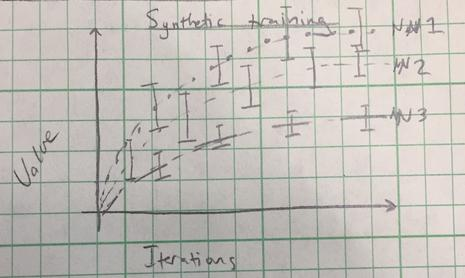
\includegraphics[width=0.9\textwidth]{Images/ToySyntheticTrainingAccuracy.jpg}
    \caption{Training progress of cost function}
    \label{fig:ToySyntheticTraningAccuracy}
\end{figure}

\begin{figure}[h]
    \centering
    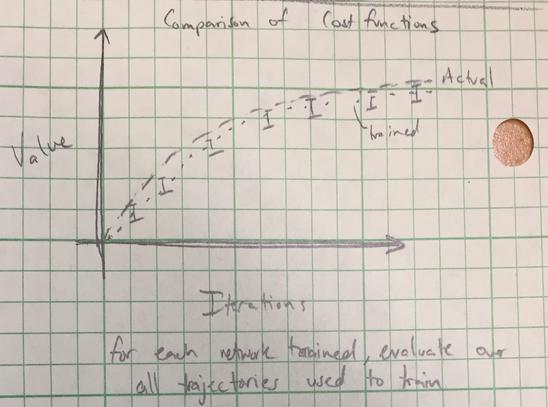
\includegraphics[width=0.9\textwidth]{Images/ToySyntheticCostComparison.jpg}
    \caption{Comparison of trained cost function to actual cost function.}
    \label{fig:ToySyntheticCostComparison}
\end{figure}

\begin{figure}[h]
    \centering
    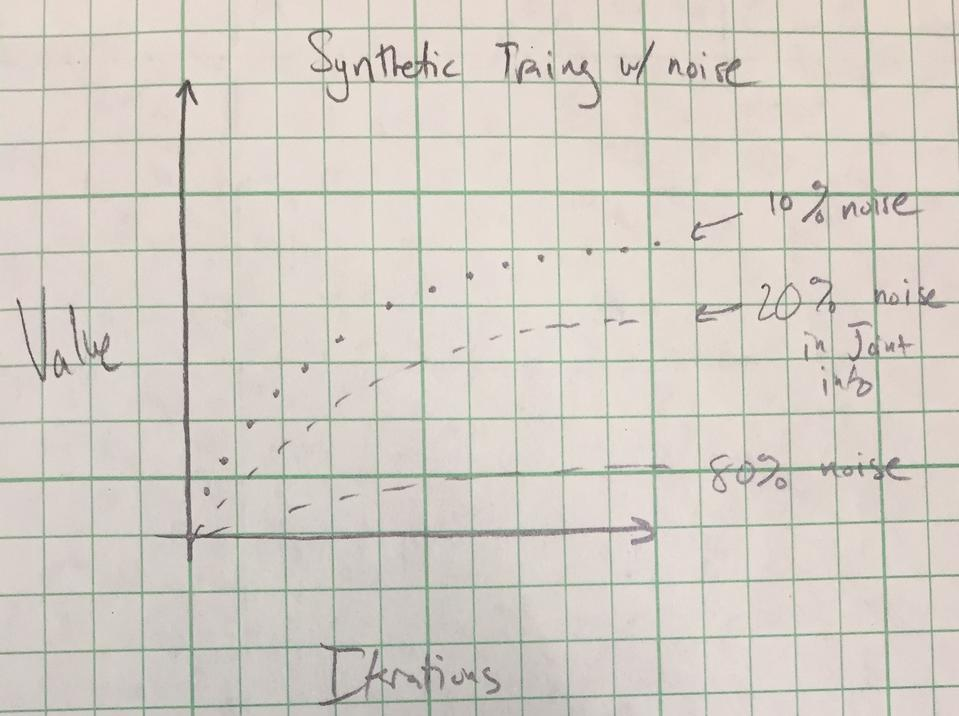
\includegraphics[width=0.9\textwidth]{Images/ToySyntheticNoise.jpg}
    \caption{Comparison of trained cost functions with different amounts of noise.}
    \label{fig:ToySyntheticNoise}
\end{figure}

\subsection{Human Training}

\begin{figure}[h]
    \centering
    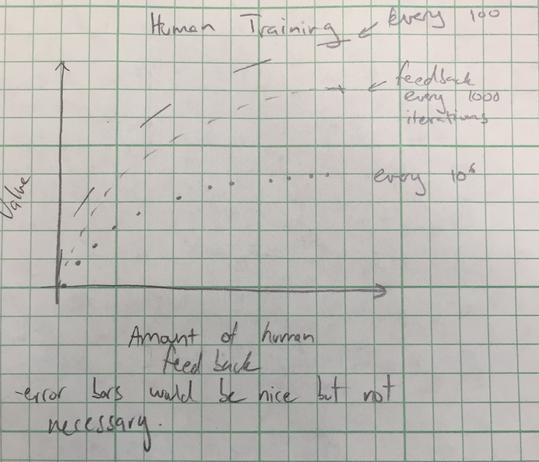
\includegraphics[width=0.9\textwidth]{Images/ToyHumanTrainingProgress.jpg}
    \caption{Training progress of cost function with human feedback.}
    \label{fig:ToyHumanTraningProgress}
\end{figure}

\begin{figure}[h]
    \centering
    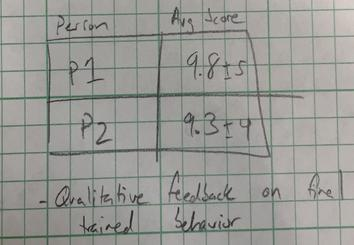
\includegraphics[width=0.9\textwidth]{Images/ToyHumanCostComparison.jpg}
    \caption{Qualitative estimate of how much a person agrees with the goal behavior.}
    \label{fig:ToyHumanCostComparison}
\end{figure}


\subsection{Combined Training}
\begin{figure}[h]
    \centering
    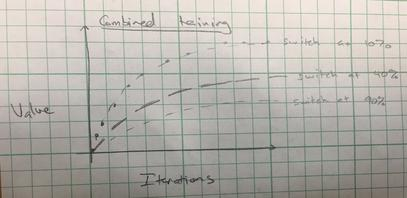
\includegraphics[width=0.9\textwidth]{Images/ToyCombinedTraining.jpg}
    \caption{Training progress of cost function with synthetic feedback followed by human feedback.}
    \label{fig:ToyCombinedTraningProgress}
\end{figure}


\subsection{Grasping Domain}
Grasping domain is turning a handle.  Software used is OpenRAVE.  Ported over same framework.

\begin{figure}[h]
    \centering
    
\includegraphics[width=0.25\textwidth]{Images/placeholder.png}
    \caption{Training progress of cost function}
    \label{fig:GraspingSyntheticTraningAccuracy}
\end{figure}

\begin{figure}[h]
    \centering
    
\includegraphics[width=0.25\textwidth]{Images/placeholder.png}
    \caption{Training progress of cost function}
    \label{fig:GraspingCombininedTraningProgress}
\end{figure}